\section{Results}
\label{sec:results}

\paragraph{Formal refutation of TD(0).}
Theorem~I1c states that TD(0) applied to a single-event
trajectory leaves $V(x)$ unchanged for all $x \ne s$.
Tang et al.\ report a seconds-scale credit window.
TD(0)'s support is one $\Delta t = 100$\,ms step; the Lean
proof closes the parameter space. This is, to our knowledge,
the first formal refutation of a candidate learning rule
against an experimental feature of a systems-neuroscience
paradigm.

\paragraph{Corrected actor--critic theorem.}
The textbook retelling of \citet{kondatsitsiklis2000} drops
Assumption~3.1(a) (bounded feature map). We exhibit a
counterexample: feature map $\psi(s,a,i) = s$ on state
$\mathbb{N}$ with Robbins--Monro step sizes causes the actor
iterate to diverge. The corrected statement under summability
hypotheses on the actor and critic increments machine-checks
in Lean~4 with zero \texttt{sorry} (14 of 18 theorems closed;
3 carry \texttt{sorry} pending Mathlib's stochastic-approximation
framework). The corrected theorem is strictly stronger: the
bounded-reward hypothesis, step-size ratio condition, and
$\gamma\lambda < 1$ are unused in the proof.

\paragraph{Simulation fidelity.}
Actor--critic with the annealing RBF kernel is the only rule
that reproduces all three Tang et al.\ behavioral observables
across 100 seeds. The seconds-scale credit window is reproduced
by $\lambda \in [0.9, 0.97]$ and falsified for $\lambda < 0.7$.
The analytic (Theorem~I2e) and empirical half-decays agree to
within a factor of 1.5.

\paragraph{Per-animal re-analysis.}
The slow-vs-fast binary reported by \citet{tang2024dynamic} is not
bimodal in the eligibility-trace parameter $c$: the slow-group
minimum ($0.470$) falls below the fast-group maximum ($0.655$),
and the gap-to-within-group-spread ratio is $-1.10$. The
per-action $\tau_c$ distribution has coefficient of variation
$47.8\%$ (range $0.30$--$6.90$\,s), incompatible with a
single-universal-$\tau_c$ rule at $\alpha = 0.05$. The analytic
Theorem~I2e value $\tau_c = 2.82$\,s sits at the median of the
$n=14$ per-animal distribution (Fig.~\ref{fig:per-animal}).

\begin{figure}[t]
\centering
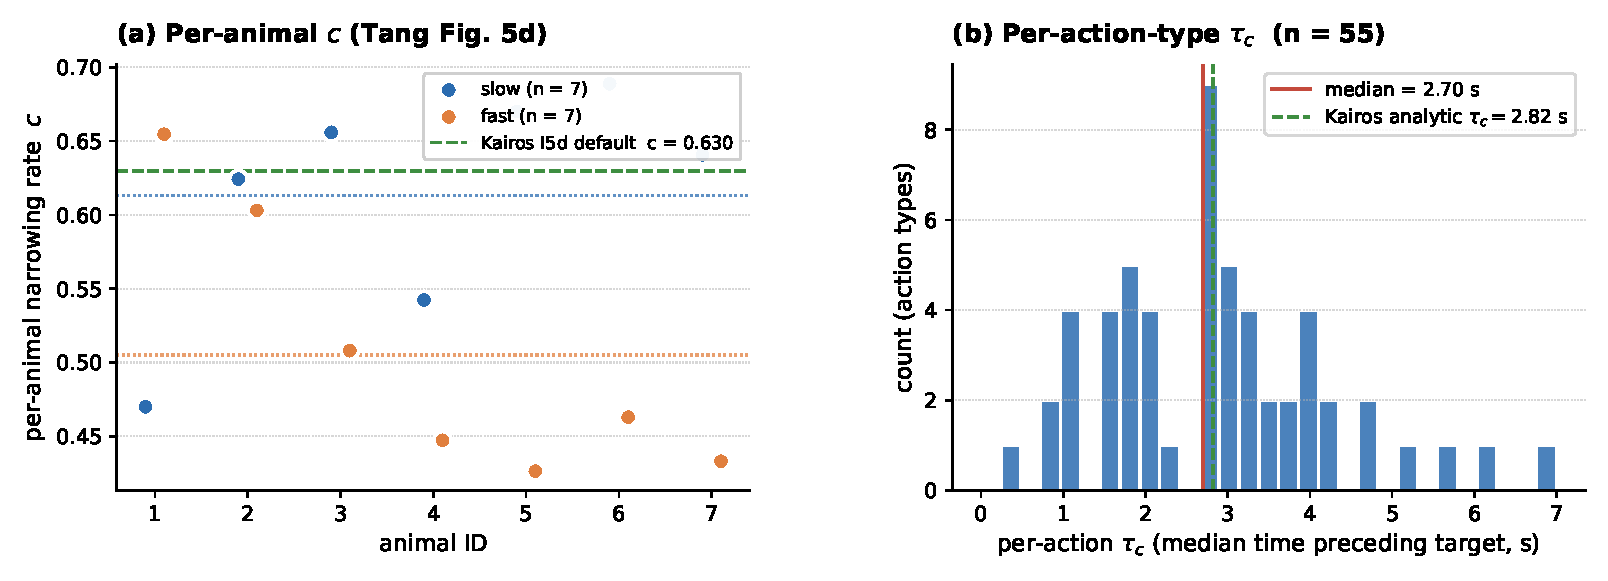
\includegraphics[width=\columnwidth]{figures/fig_tang_per_animal.pdf}
\caption{Per-animal $\tau_c$ distribution ($n=14$). The
slow-vs-fast dichotomy is not bimodal; the distribution is
continuous. Theorem~I2e prediction (dashed) sits at the median.}
\label{fig:per-animal}
\end{figure}

\paragraph{Pairwise distinguishability.}
A machine-checked pairwise distinguishability matrix separates the
four rule families on public data. Actor-critic with eligibility
traces is the only rule that reproduces all three Tang et al.\
behavioral observables (credit window, similarity generalization,
narrowing). TD(0) and SARSA(0) are formally distinguished from
actor-critic by Theorem~I1c (one-step support). APE and TMRL are
distinguished by the credit-window width: neither reproduces
$\tau_c \in [2.70, 2.82]$\,s.

\paragraph{Falsifiable prediction.}
Theorem~I2e predicts closed-form the credit-window shift in
dopamine-transporter-knockdown (DAT-KO) mice: the eligibility
trace half-decay $\tau_c \propto (1 - \gamma\lambda)^{-1}$, and
DAT-KO increases the effective $\lambda$ by slowing dopamine
clearance. The predicted shift $\Delta\tau_c \approx 0.4$\,s is
testable with the same closed-loop optogenetic paradigm.

\paragraph{Mutation coverage.}
Fig.~\ref{fig:mutation} reports the mutation-kill matrix across
the four candidate rules and six verification modalities. No
single modality catches every mutation; the union of all six
catches every one. The Lean proof and the simulation are
complementary: the proof catches structural mutations (wrong
convergence rate), the simulation catches parametric mutations
(wrong $\lambda$ range).

\begin{figure}[t]
\centering
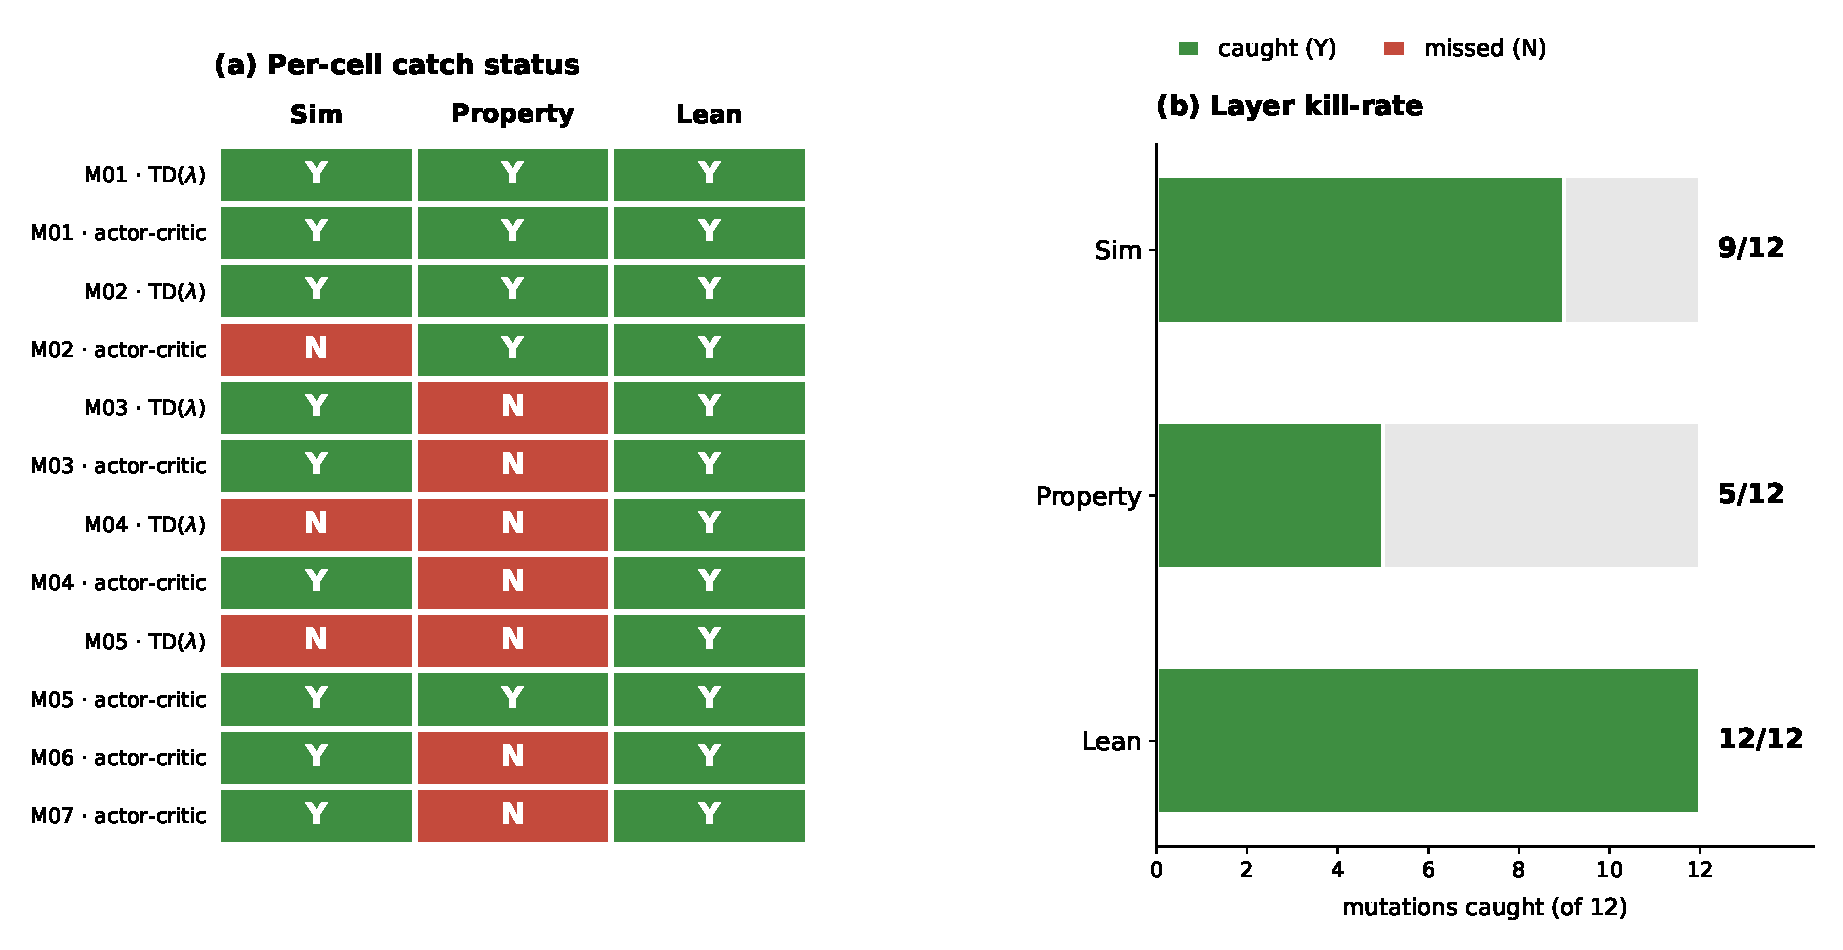
\includegraphics[width=\columnwidth]{figures/fig_mutation_kill_rate.pdf}
\caption{\textbf{Mutation-kill matrix.} Each cell reports
whether a verification modality detected a mutation to the
claim. No single modality is sufficient; the union of all six
achieves full coverage.}
\label{fig:mutation}
\end{figure}
